\section{Experimental Results}
\label{sec:experimentalResults}
\todo[inline]{Display results in suitable representation.}
\todo[inline]{Choose what to present}
\begin{itemize}
\item For each experiment
\item Present setup.
\item model layering. Same. Reasons. Gave good results on their own.
\end{itemize}

\todo[inline]{Or put this in it's own chapter}
\todo[inline]{Avoid drawing grand conclusions. Only what your data can support}
\todo[inline]{Study tables graphs for unusual things that might raise questions with the reader}

The performance of the system has not been compared to \citep{saito_building_and_roads} and \citep{Mnih_aerial_images_noisy}, due to the fact that the precision and recall metrics described in Section \ref{sec:background_theory} have not been implemented yet.\\

Nonetheless, the center image in Figure \ref{fig:result} illustrates the current performance of the system. In this particular test image, the model is able to identify the majority of the roads present, except for a small gravel road on the right side of the image. There are also a lot of prediction errors, such as roads being disconnected, and prediction artefacts in the forest areas. An interesting observation is that the model also correctly predicts small private roads leading up to houses present in the image. Furthermore, the model detects construction roads in the upper left corner. Since these roads are not present in the label image, the model is penalized for these predictions by the cross-entropy loss function.\\


\begin{figure}[t]
\centering
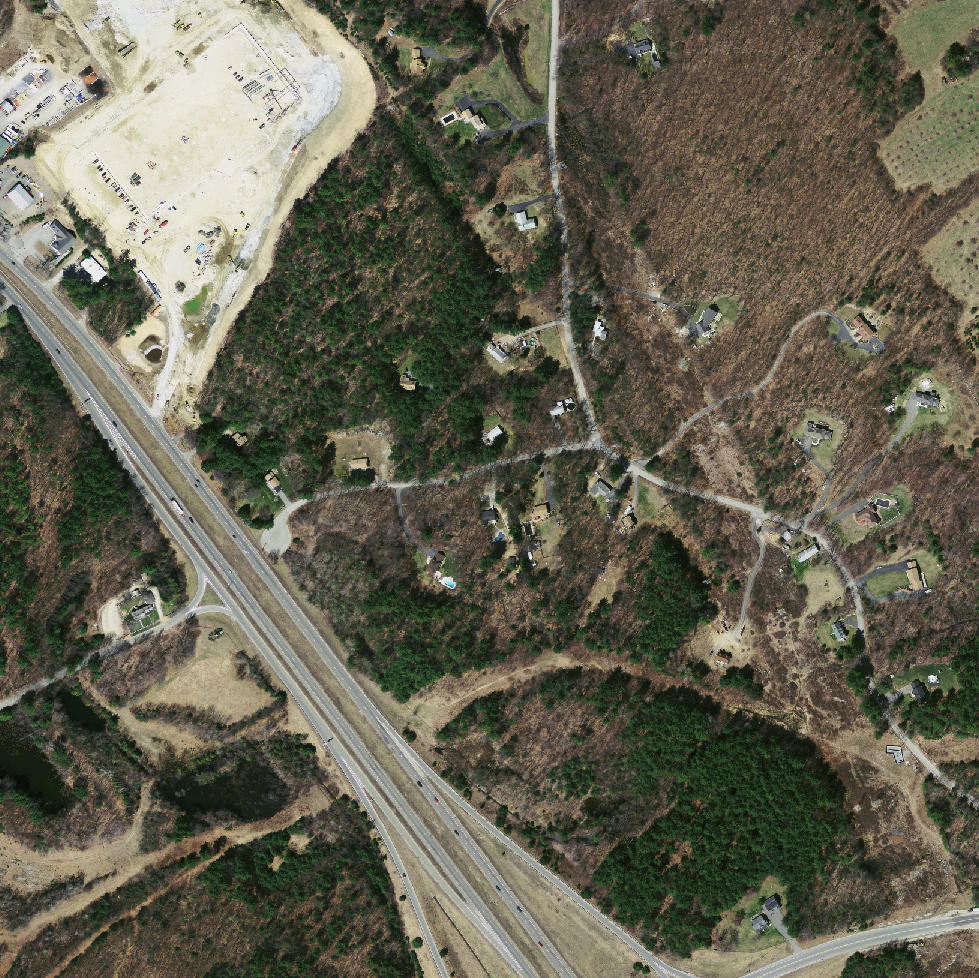
\includegraphics[width=.32\textwidth]{figs/results_data.jpg}\hfill
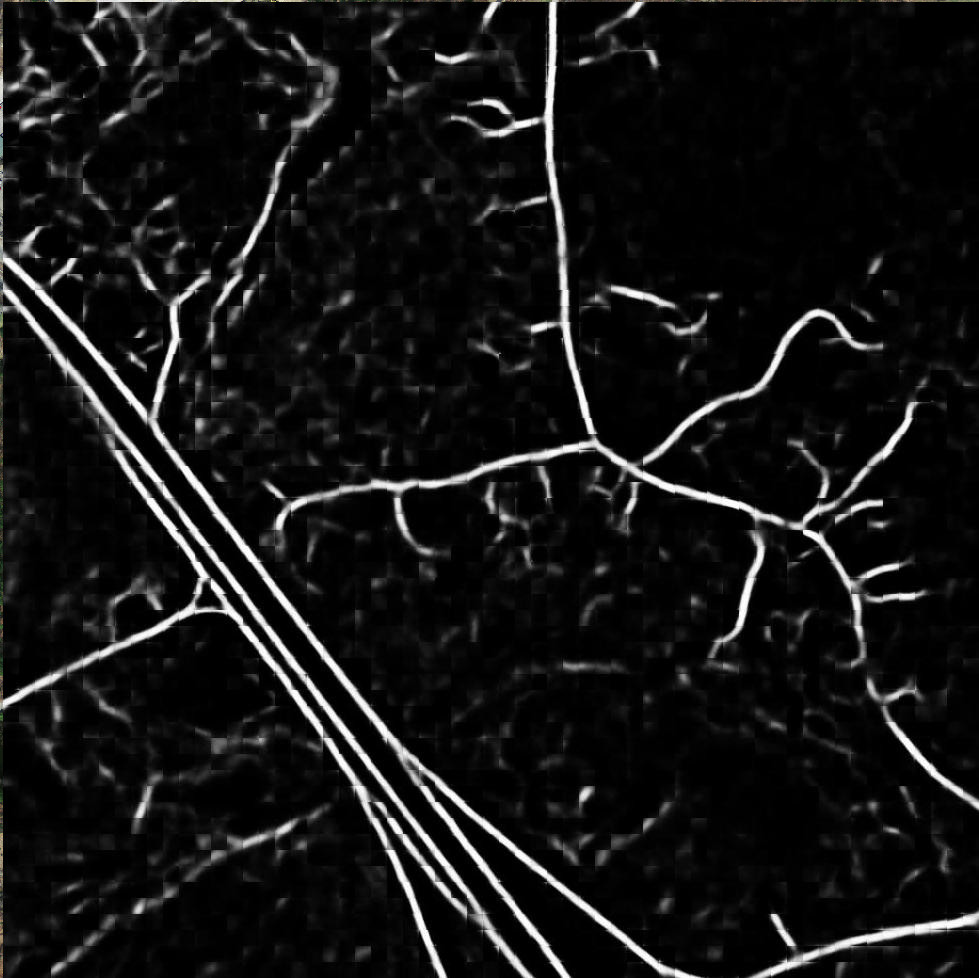
\includegraphics[width=.32\textwidth]{figs/results_label.jpg}\hfill
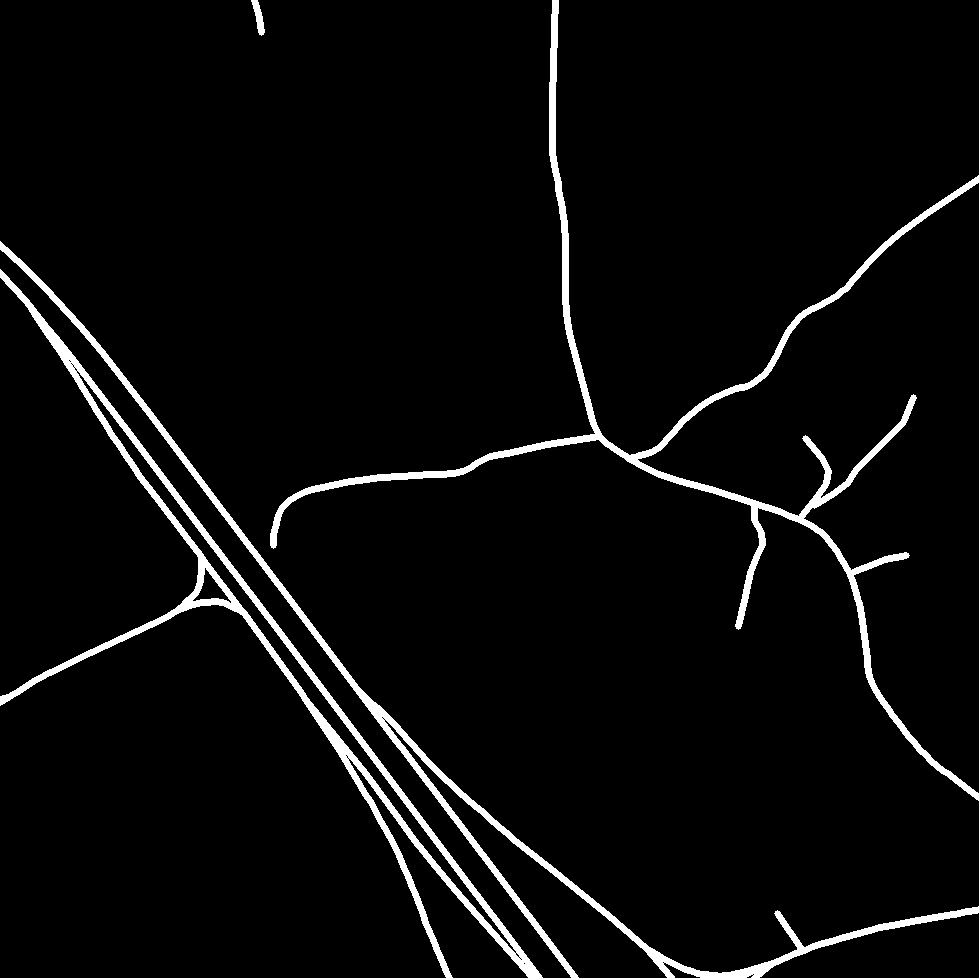
\includegraphics[width=.32\textwidth]{figs/label.png}

\caption{Aerial image, model prediction and label image. The aerial image is part of test set in Massachusetts Roads Dataset}
\label{fig:result}
\end{figure}


\begin{figure}
\begin{subfigure}{0.48\textwidth}
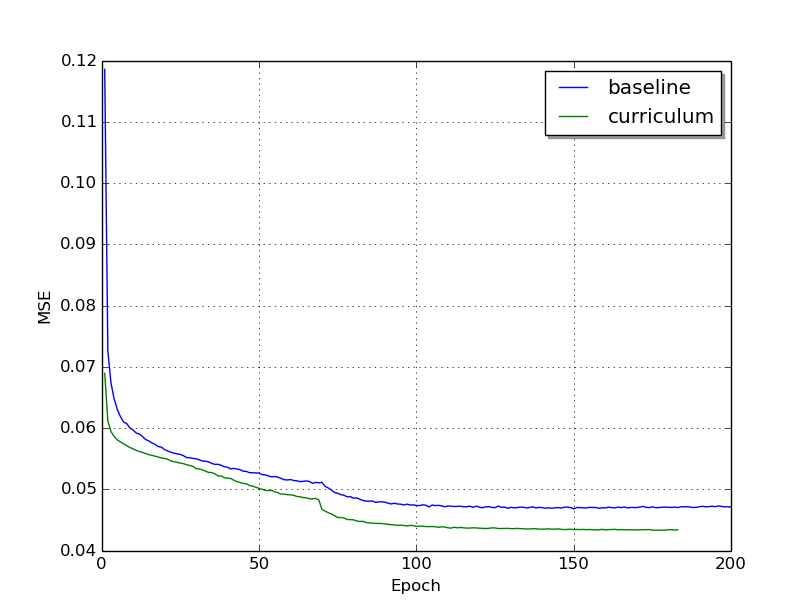
\includegraphics[width=\linewidth]{figs/curr50/loss_compare_validation.png}
\caption{Comparison of validation loss.} \label{fig:curr50_loss}
\end{subfigure}
\hspace*{\fill} % separation between the subfigures
\begin{subfigure}{0.48\textwidth}
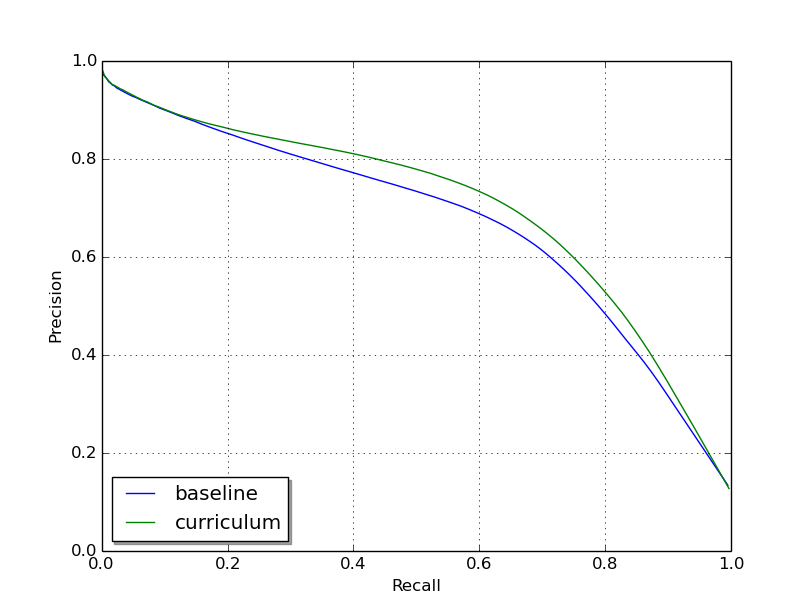
\includegraphics[width=\linewidth]{figs/curr50/validation_precision_recall_curve.png}
\caption{Precision and recall comparison.} \label{fig:curr50_pr}
\end{subfigure}
\hspace*{\fill} % separation between the subfigures
\caption{Curriculum learning, with switch after 70 epochs. Models trained with 110800 examples. 10 runs, averaged. Baseline and curriculum} \label{fig:curr50}
\end{figure}


\begin{figure}
\begin{subfigure}{0.48\textwidth}
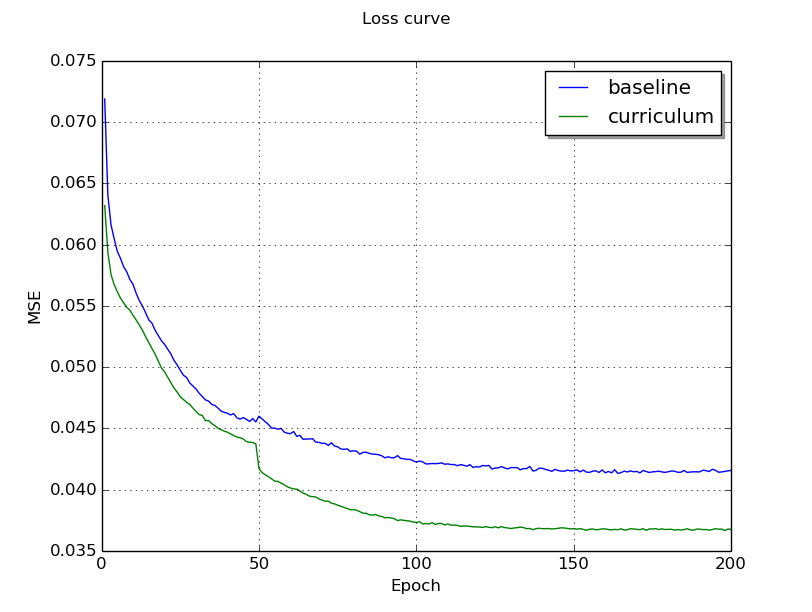
\includegraphics[width=\linewidth]{figs/curr100/validation_loss_curve.png}
\caption{Comparison of validation loss.} \label{fig:curr100_loss}
\end{subfigure}
\hspace*{\fill} % separation between the subfigures
\begin{subfigure}{0.48\textwidth}
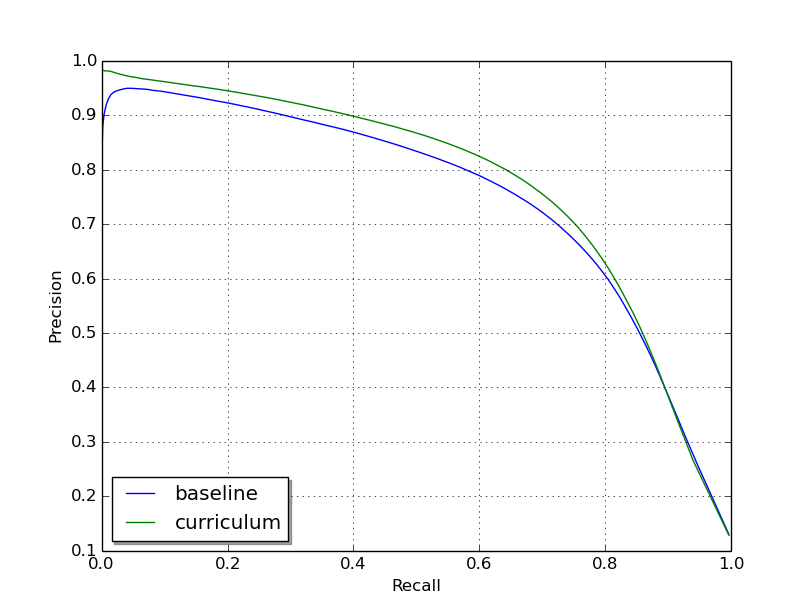
\includegraphics[width=\linewidth]{figs/curr100/validation_precision_recall.png}
\caption{Precision and recall comparison.} \label{fig:curr100_pr}
\end{subfigure}
\hspace*{\fill} % separation between the subfigures
\caption{Curriculum learning, with switch after 50 epochs. Models trained with 221600 examples. 10 runs, averaged} \label{fig:curr100}
\end{figure}


\begin{figure}
\begin{subfigure}{0.48\textwidth}
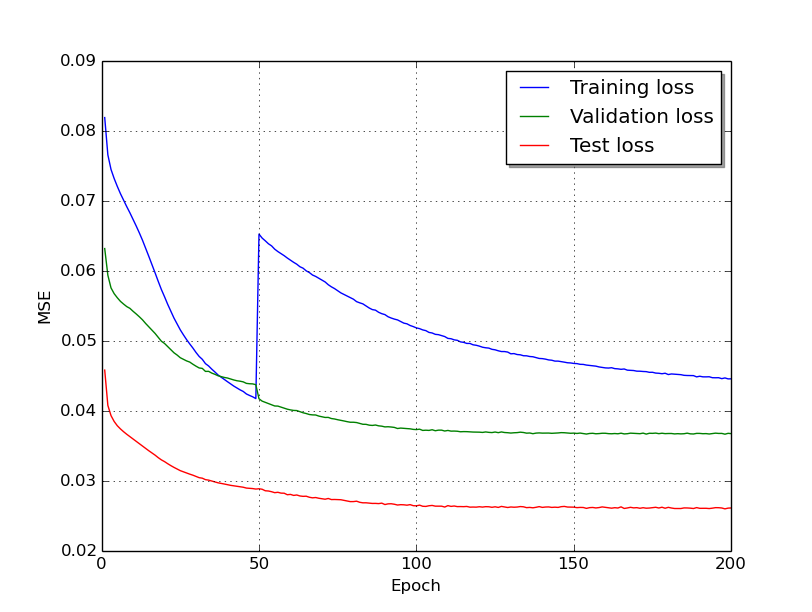
\includegraphics[width=\linewidth]{figs/curr100/curriculum_loss_curves.png}
\caption{Curriculum loss.} \label{fig:curr100_loss2}
\end{subfigure}
\hspace*{\fill} % separation between the subfigures
\begin{subfigure}{0.48\textwidth}
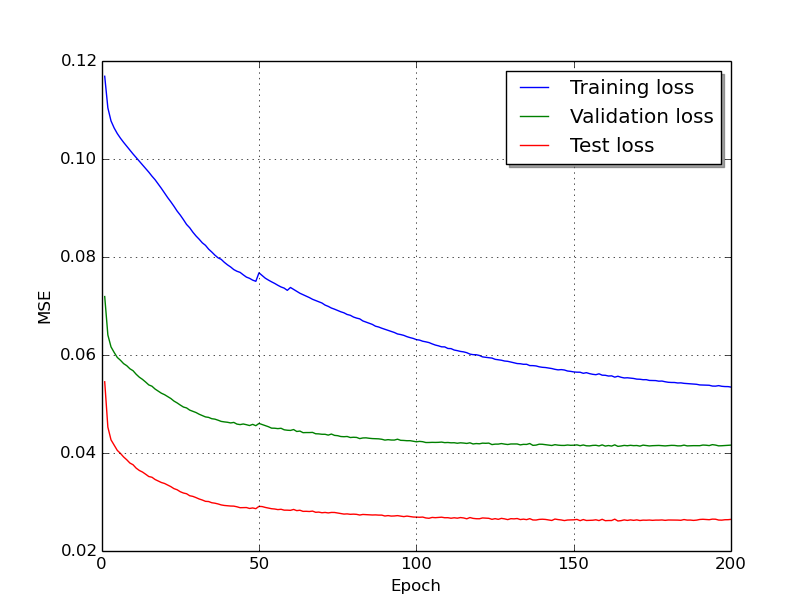
\includegraphics[width=\linewidth]{figs/curr100/baseline_loss_curves.png}
\caption{Baseline loss.} \label{fig:curr100_epochs_baseline2}
\end{subfigure}
\hspace*{\fill} % separation between the subfigures
\caption{Loss for training, validation and test dataset. 221600 examples.} \label{fig:curr100_loss_epochs}
\end{figure}
